\begin{surferPage}[15개의 뾰족점]{15개의 뾰족점을 갖는 $5$차식}
이 $5$차 곡면은 $15$개의 $A_2$ 타입(뾰족점) 특이점을 갖습니다. 이 $5$차식과 이와 관련된 곡면들은 2005년 Oliver Labs의 논문에서 소개되었습니다. $5$개의 뾰족점은 다른 $10$개와는 다른 모양을 가지고 있습니다. $5$개는 $A_2^{++}$ 타입 특이점, 나머지 $10$개는 $A_2^{+-}$ 타입 특이점입니다.

     \vspace*{-0.3em}
    \begin{center}
      \begin{tabular}{c@{\qquad}c}
        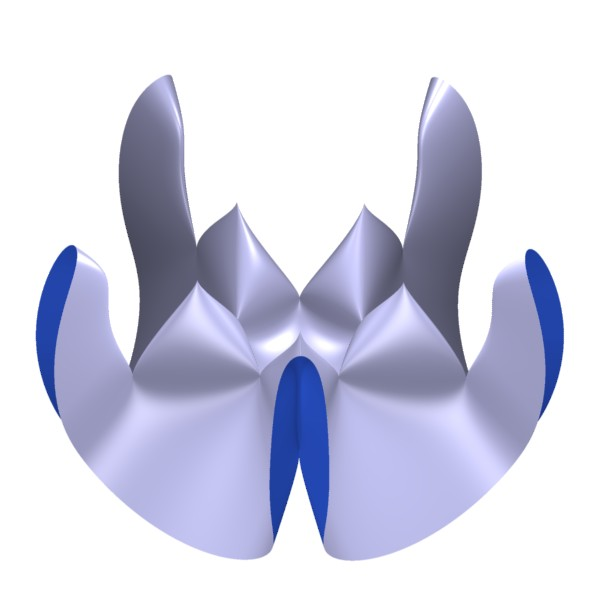
\includegraphics[height=1.2cm]{dessins_quint_15a2}
        &
        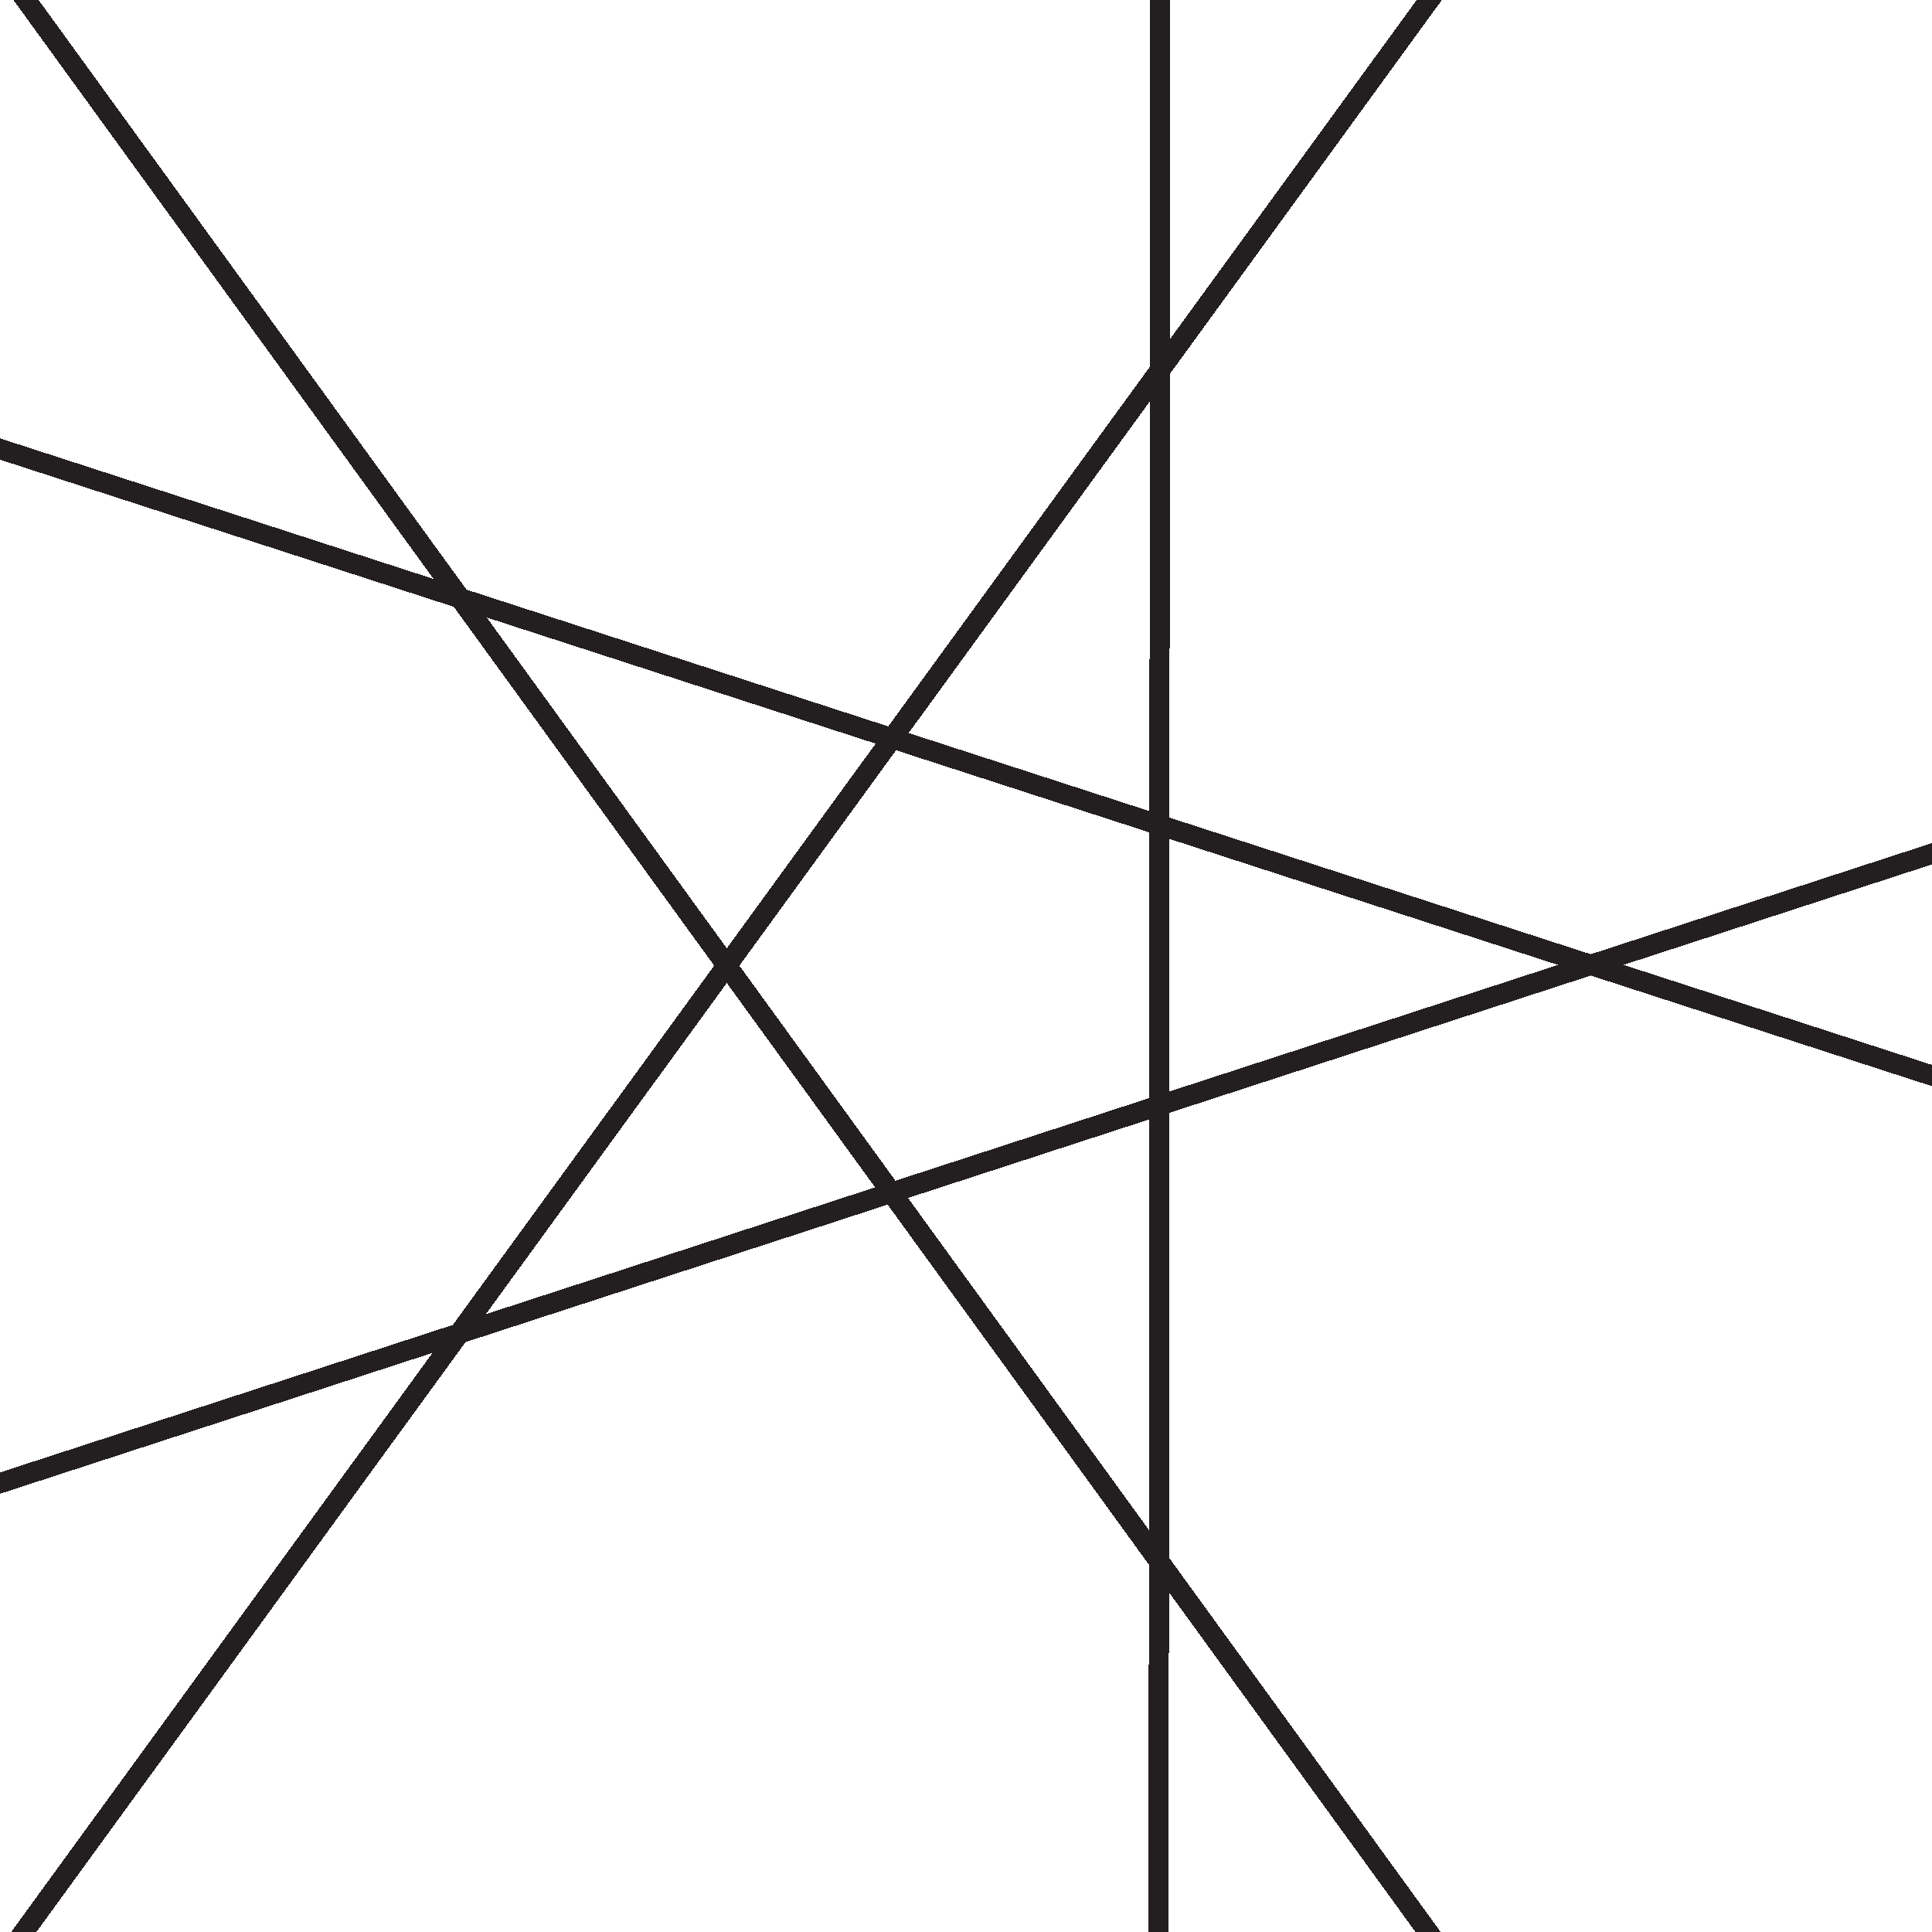
\includegraphics[height=1.2cm]{rp5.pdf}
      \end{tabular}
    \end{center}
    \vspace*{-0.3em}    
    
    이 곡면의 방정식은 아래의 형태로 쓰여질 수 있습니다. \\
    \begin{equation*}S_5(x,y) + t(z)=0
    \end{equation*}

    여기서 $S_5(x,y)$는 일반적인 오각형 그리고 $t(z)$는 이미 여러번 언급된 체비셰프 다항식의 변형된 형태입니다. 

    아래에서 왼쪽에 있는 $15$개의 특이점을 갖는 또다른 $5$차식은 울프 바스에 의해 만들어졌습니다. 이것은 가운데 그림에서 확인할 수 있듯이 오른쪽에 있는 클레브슈 $3$차식과 관련이 있습니다. 

    \vspace*{-0.3em}
    \begin{center}
      \begin{tabular}{c@{\quad}c@{\quad}c}
        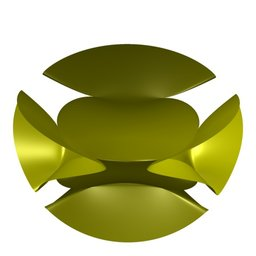
\includegraphics[height=1.2cm]{barthquintic_green}
        &
        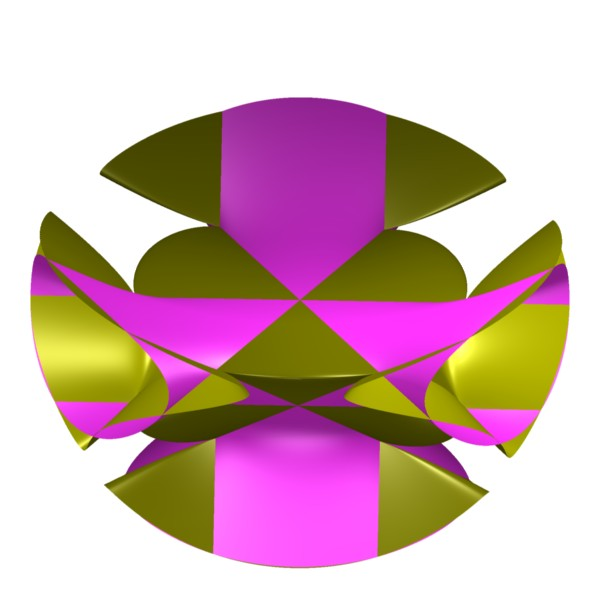
\includegraphics[height=1.2cm]{barthquintic_clebschcubic}
        &
        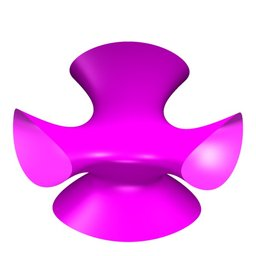
\includegraphics[height=1.2cm]{clebschcubic_pink}
      \end{tabular}
    \end{center}
\end{surferPage}
